\documentclass[twoside,11pt]{article}

\usepackage{amsmath}
\usepackage{bm}
\usepackage{comment}

\usepackage{graphicx, subcaption}

\usepackage{tikz}

\usetikzlibrary{bayesnet}

\pgfdeclarelayer{edgelayer}
\pgfdeclarelayer{nodelayer}
\pgfsetlayers{edgelayer,nodelayer,main}

\definecolor{hexcolor0xbfbfbf}{rgb}{0.749,0.749,0.749}

\tikzset{>=latex}
\tikzstyle{none}   = [inner sep=0pt]

\tikzstyle{line}  = [ - ]
\tikzstyle{arrow}  = [ ->, shorten <=1pt, shorten >=1pt ]
\tikzstyle{ardash} = [ dotted, ->, shorten <=1pt, shorten >=1pt ]

\tikzstyle{empty}=[circle,opacity=0.0,text opacity=1.0,inner sep=0pt,minimum
width=0pt,minimum height=0pt]
\tikzstyle{box}=[rectangle,fill=White,draw=Black]
\tikzstyle{filled}=[circle,fill=hexcolor0xbfbfbf,draw=Black]
\tikzstyle{hollow}=[circle,fill=White,draw=Black]
\tikzstyle{param}=[rectangle,fill=Black,draw=Black,inner sep=0pt,minimum width=4pt,minimum height=4pt]


\begin{document}
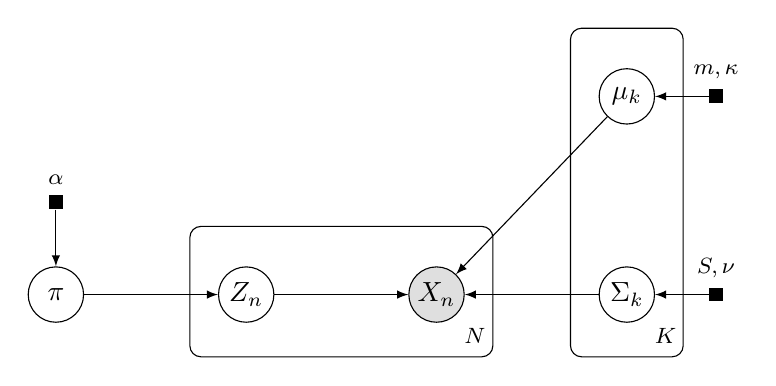
\begin{tikzpicture}[x=1.7cm,y=1.8cm]

  % Nodes
  \node[latent] (sigma) {$\Sigma_k$} ;
  \node[latent, above=of sigma] (mu) {$\mu_k$} ;
  \node[obs, left= of sigma] (X) {$X_n$} ;
  \node[latent, left= of X] (Z) {$Z_n$} ;
  \node[latent, left= of Z] (pi) {$\pi$} ;
  
  \factor[above=of pi] {alpha} {$\alpha$} {} {} ;
  \factor[right=of mu] {m} {$m, \kappa$} {} {} ;
  \factor[right=of sigma] {S}{$S, \nu $} {} {} ;

  \edge{alpha}{pi}
  \edge{pi}{Z}
  \edge{Z}{X}
  \edge{mu}{X}
  \edge{m}{mu}
  \edge{sigma}{X}
  \edge{S}{sigma}

  
  \plate[inner sep=0.35cm, yshift=0.15cm,
    label={[xshift=-14pt,yshift=14pt]south east:$N$}] {plate1} {
    (Z)(X)
  } {};
  
 \plate[inner sep=0.35cm, yshift=0.15cm,
    label={[xshift=-14pt,yshift=14pt]south east:$K$}] {plate1} {
    (mu)(sigma)
  } {};

  
\end{tikzpicture}

\begin{comment}
% example figure for reference
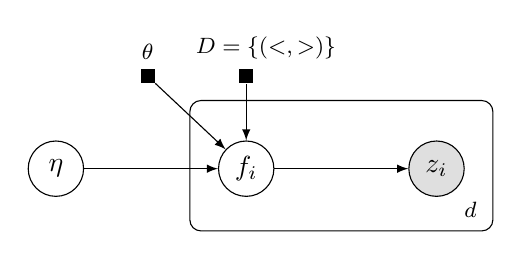
\begin{tikzpicture}[x=1.7cm,y=1.8cm]

  \node[obs]                  (z)      {$z_i$} ;
  \node[latent, left=of z]    (f)      {$f_i$} ;
  \node[latent, left=of f]    (xi)      {$\eta$} ;

  \factor[above=of f, xshift=-1.25cm] {theta} {$\theta$} {} {};
  \factor[above=of f] {D} {\hspace{0.5cm}$D=\{(<,>)\}$} {} {};
  %\factor[above=of f] {D} {$\mathcal{D}$} {} {};

  % Edges
  \edge{xi}{f};
  \edge{f}{z};
  \edge{theta}{f};
  \edge{D}{f};

  % Plates
  \plate[inner sep=0.35cm, yshift=0.15cm,
    label={[xshift=-14pt,yshift=14pt]south east:$d$}] {plate1} {
    (z)(f)
  } {};

\end{tikzpicture}
\end{comment}

\end{document} 



































